\begin{figure}[t]
\centering
% 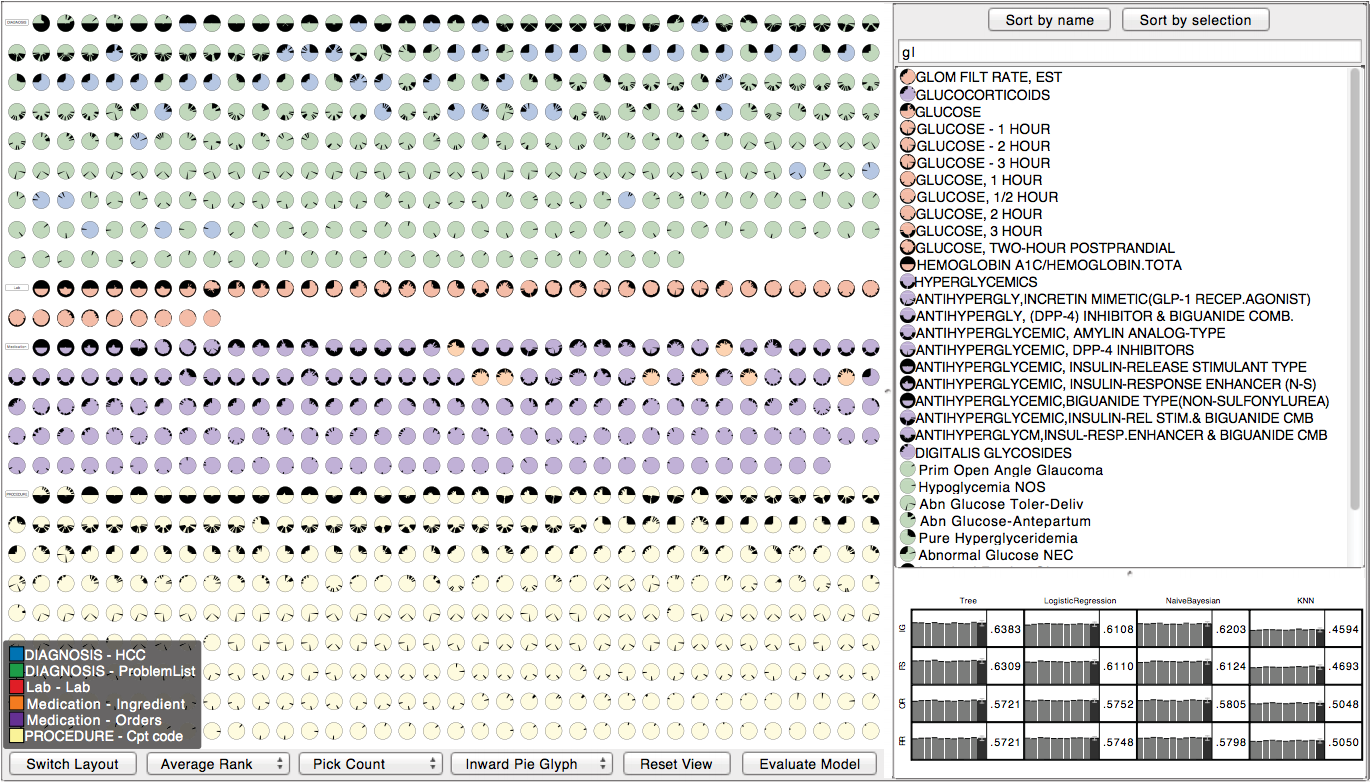
\includegraphics[scale=0.32]{fig/overview}
% ~
% \includegraphics[scale=0.32]{fig/confusion}
% ~
% 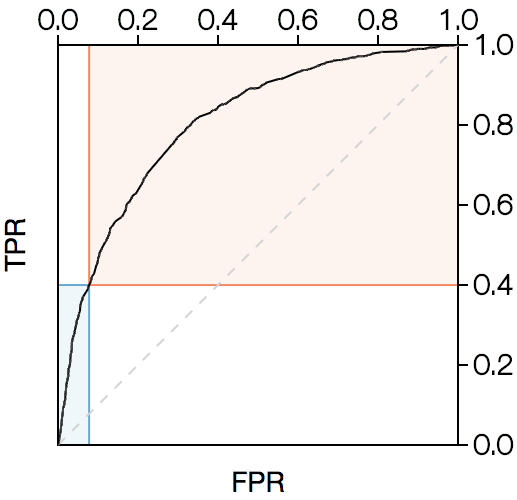
\includegraphics[scale=0.32]{fig/roc}
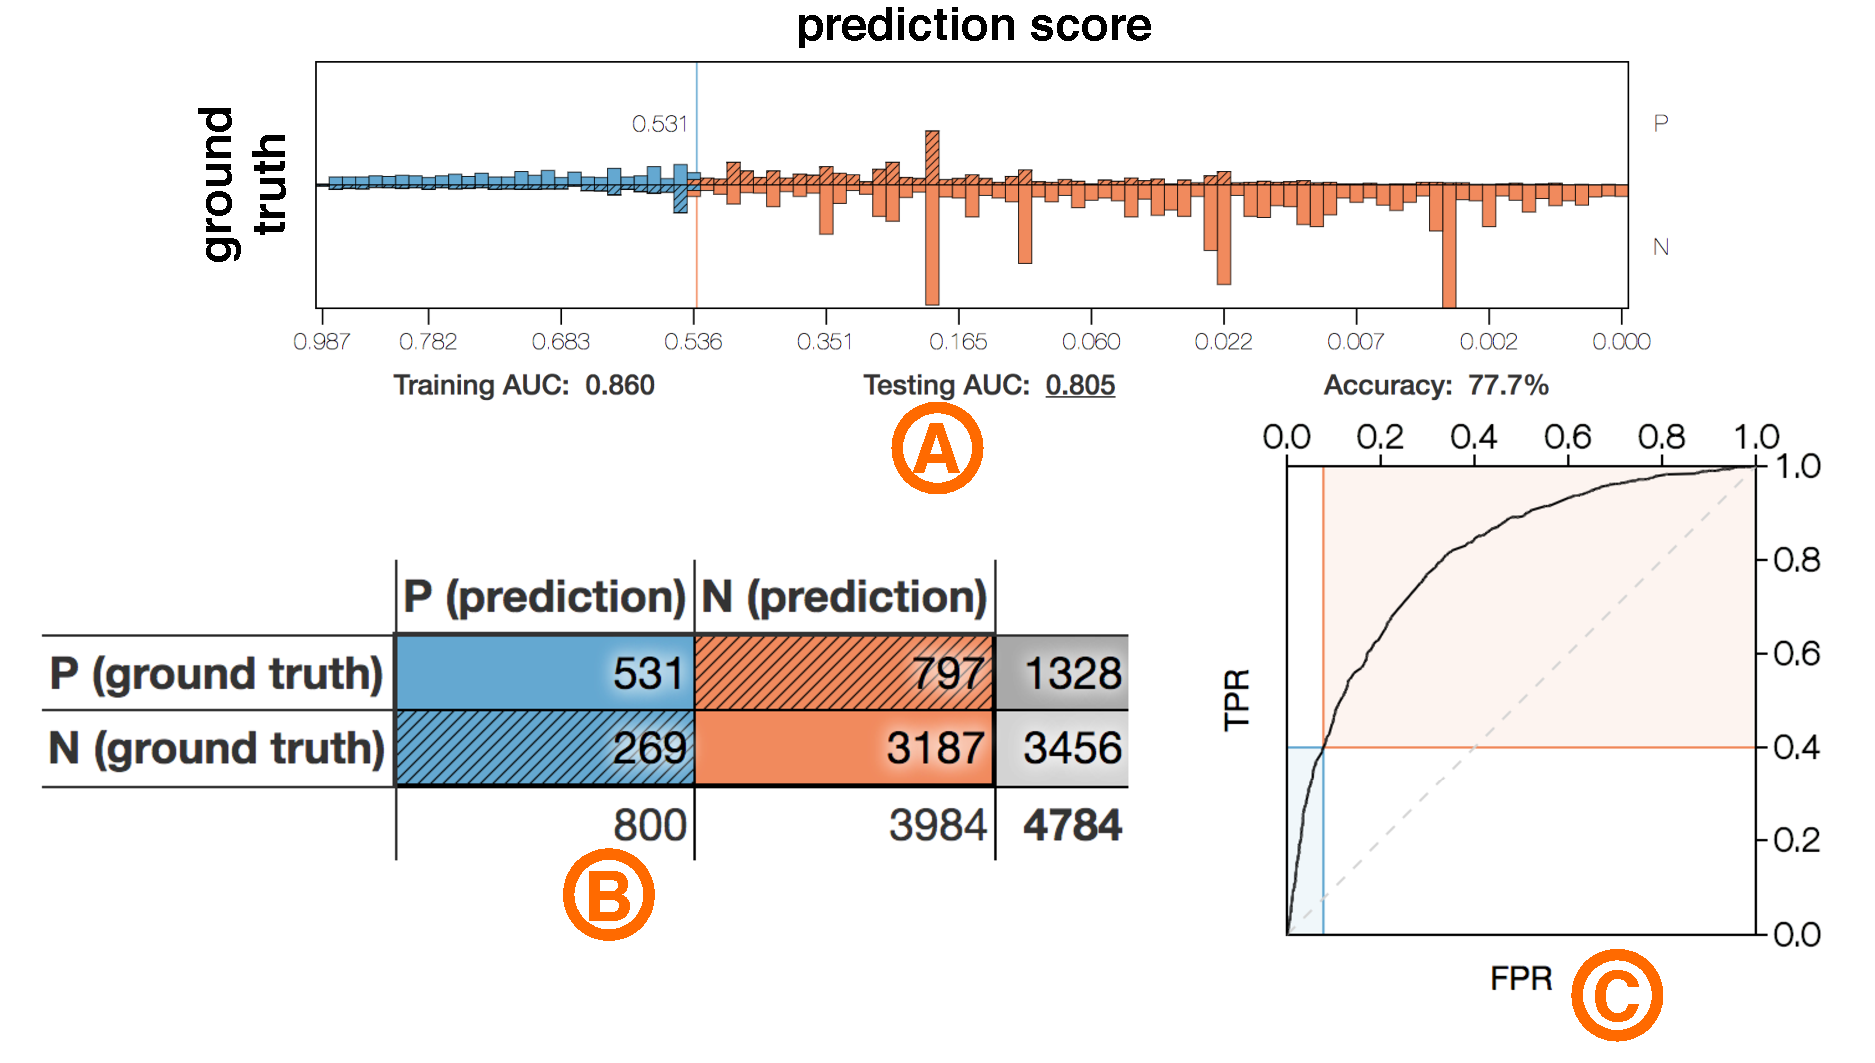
\includegraphics[width=\columnwidth]{explainer/overview_final}
\vspace{-8mm}
\caption{
The \textbf{\tabA}.
(A) Histograms showing the distribution of prediction scores.
The direction of the bars indicates the ground truth and their position relative to the threshold line (at 0.531) indicates the predicted label.
(B) The confusion matrix shows the number of correct and incorrect predictions. (C) The ROC curve shows the prediction quality.
}
\vspace{-5mm}
\label{figs:overview}
\end{figure}

% Selecting the peak left of 0.165 reveals ``Sodium Chloride" as its main cause in the \tabB. 

\begin{figure}
\centering
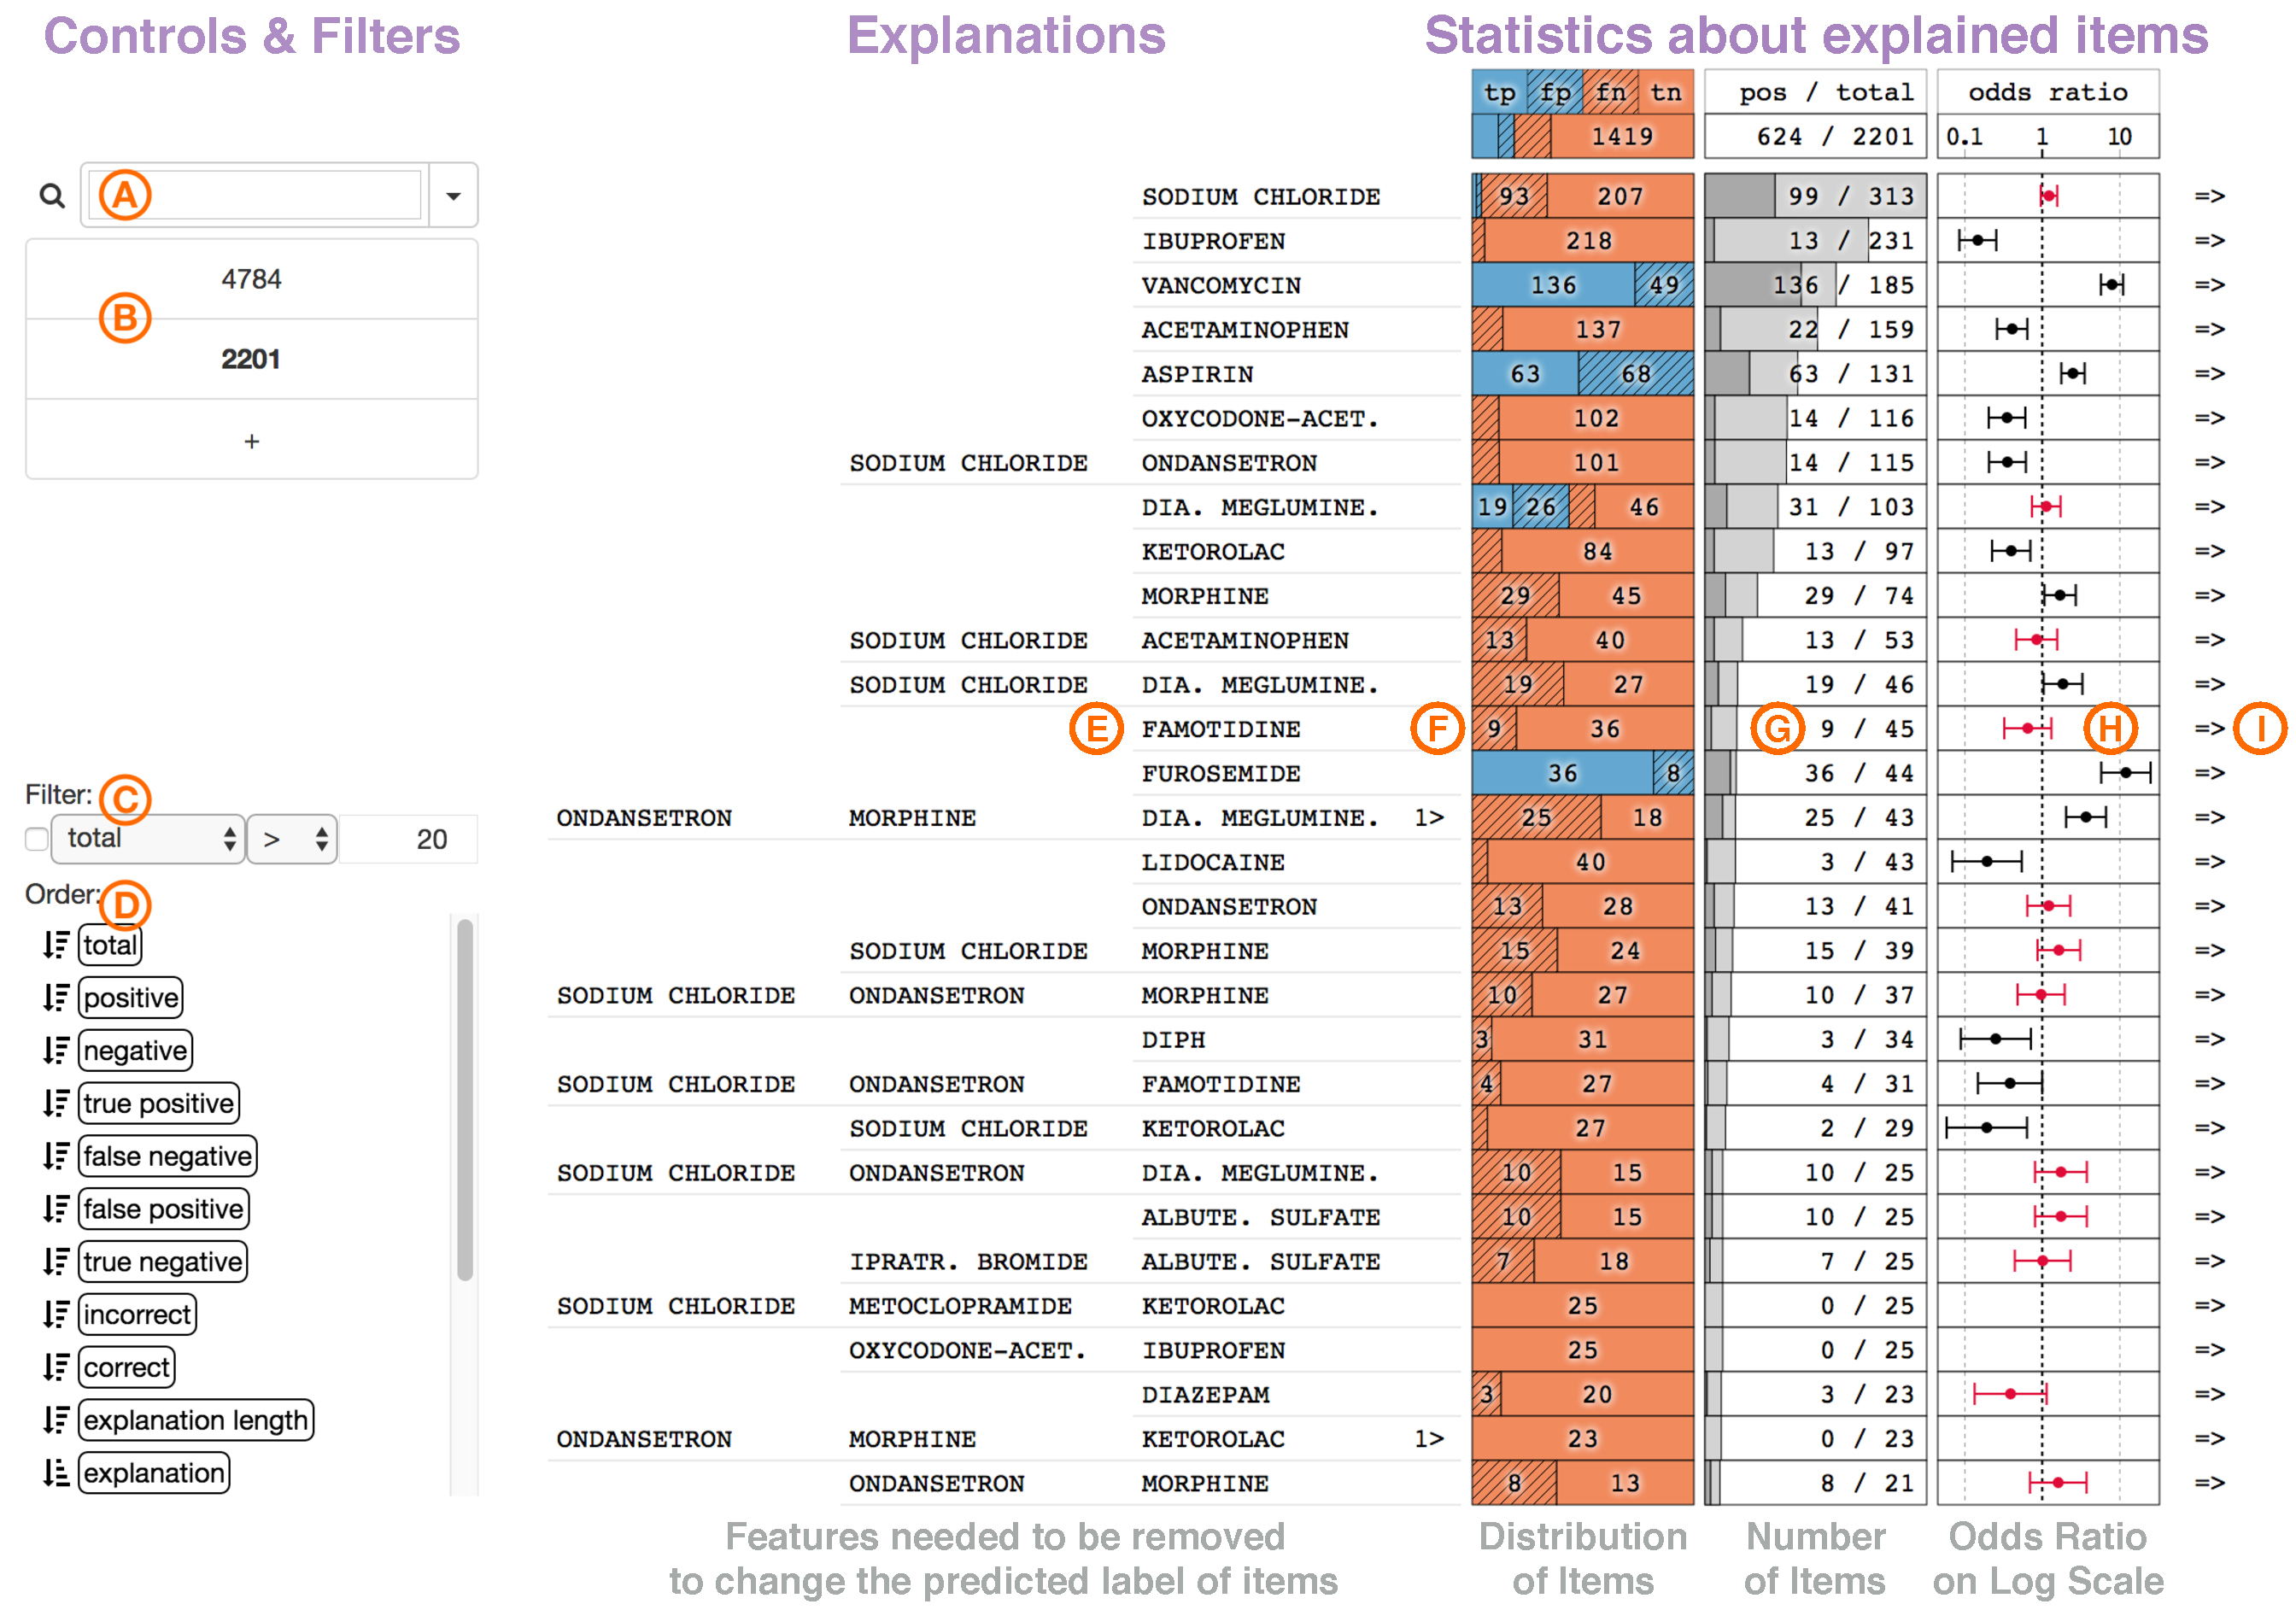
\includegraphics[width=0.8\linewidth]{explainer/controlexplain}%
\raisebox{2.05em}{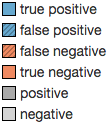
\includegraphics[height=6.9em]{explainer/iamlegend}}
\caption[The \tabB.]{
In the \textbf{\tabB} each row represents a group of data items explained by a set of features (E).
An indicator is shown for explanations longer than 3 features.
Column (F) shows the distribution of true / false positive / negative data items within the group.
Colors show the predicted label (``blue" for positive and ``orange" for negative) and a hatching pattern indicates incorrect predictions.
Column (G) shows the number of items captured by the explanation.
The bars are relative to the size of the largest explanation.
Column (H) shows the odds ratio of the group on a logarithmic scale.
Whiskers show the confidence interval.
The arrows on the right (I) navigate to the \tabC focusing on the given explanation. The controls of the \tabB are shown on the left.
The first entry of the list of filtered data items (B) represents the full dataset and following entries show sizes after filter steps are applied.
The ``+" creates a new filter according to the current selection of explanations.
Explanations can be selected satisfying a condition (C) or by searching for features in the search box (A).
The sort order of explanations is defined by the list at the bottom (D).
}
\label{figs:expl_main}
\end{figure}

\section{Visual Interface}
\label{sec:ui}
Our proposed user interface\footnote{\href{https://github.com/nyuvis/explanation_explorer}{https://github.com/nyuvis/explanation\_explorer}} consists of three different panels, each corresponding to the different goals of our proposed workflow that we described in Section~\ref{sec:model-diagnostics}. By interacting with each panel and navigating across these panels, experts can diagnose different aspects of model behavior.
% The panels are shown at the top and a user can freely navigate between those views.

In the visualizations that are a part of our interface, 
the colors orange and blue are used to show negative and positive \textit{prediction} quantities.
A hatching pattern is used for quantities where those predictions are \textit{incorrect} according to the ground truth of the data.
In this section, we describe each panel according to the order of the workflow: \tabA of the machine learning model, the \tabB, and the \tabC.

\subsection{Statistical Summary View}

% The first panel shows the \tabA of the machine learning model (see Figure~\ref{figs:overview}).
The purpose of this panel~(Figure~\ref{figs:overview}) is to address \textbf{G1} by providing a quick summary of the performance of a trained model that can help detect shortcomings before proceeding with further analyses of the model. 
% aritra commented out as I think this is not necessary: and instead changing hyper-parameters or modeling techniques.
The view consists of multiple components.

The histograms~(Figure~\ref{figs:overview}A) show the distribution of data items over prediction scores.
The chosen threshold is shown as vertical line.
Bars going up indicate the number of predicted positive labels while bars going down show predicted negative labels as emphasized by the color of the bars.
The prediction score goes from $1$ to $0$ from left to right to match the order of cells in the confusion matrix.
Likewise, bars at the bottom, left of the threshold, and at the top, right of the threshold, depict incorrectly predicted data items as indicated by their hatching pattern.
Selecting a particular bar lets the user navigate to the \tabB for inspecting items that fall in the given range of prediction scores.

The confusion matrix~(Figure~\ref{figs:overview}B) splits data items by their ground truth (vertical) and the predicted label (horizontal).
The edge of the matrix shows the sums of its columns and rows.
The predicted label depends on a threshold that divides prediction scores into positive and negative.
We choose the threshold to minimize incorrect predictions (\ie, the threshold with the smallest number of false positive and false negative predictions).



The ROC curve on the testing data~(Figure~\ref{figs:overview}C)
shows the false positive rate ($\frac{FP}{FP + TN}$) plotted against the true positive rate ($\frac{TP}{TP + FN}$).
The thresholds for those values are implicit in the plot.
However, the position for the chosen optimal threshold (as described above) is indicated in the plot via two crossing lines.

The area under the ROC curve (AUC) is also shown for both the testing and the training data set.
An AUC of $1$ indicates optimal prediction while an AUC of $0.5$ equals classification by flipping a coin.
Comparing the training AUC to the test AUC is a good estimator of how well the given model generalizes the training data.
A very high training AUC with a much lower test AUC indicates overfitting of the training data.
In addition to the AUC the accuracy of the model with the chosen threshold is also shown.

\subsection{Explanation Explorer}

The second panel, the \tabB (Figure~\ref{figs:expl_main}),  addresses \textbf{G2} and \textbf{G3} by encoding a list of explanations based on the method we described in Section~\ref{sec:algo}. The explanations are representative of the main model decisions and the associated statistics about explained items provide insight into the accuracy of those decisions.
Each row in the list represents one subgroup of data items explained using a single explanation set.
The rows can be filtered based on different criteria for user exploration which we describe below.
The row on top shows information for the full set of current data items.

The first column of the list shows this explanation (Figure~\ref{figs:expl_main}E).
In order to make this information quickly readable we only show the first three features of an explanation and indicate if there are more features present by adding a marker, showing the number of remaining features, on the right side of the feature names.
Furthermore, the feature descriptions are abbreviated in a way that each feature takes up the same amount of space.
With this the complexity of an explanation~\ie, the number of features used in an explanation, can be seen at a glance.
% If the explanation has more than three features an indicator with a number on the right shows the number of remaining features.
The full description of all features can be seen in the tooltip when hovering over the features.
The design decision to show only up to three features stems from the fact that only short explanations can be easily interpreted and having many long explanations is usually a sign of problems with the classifier, like overfitting, and in that case, the actual features involved are less interesting.

The next column shows the relative distribution of predicted labels of the explained subset of data items as stacked bars (Figure~\ref{figs:expl_main}F).
The colors blue and orange are used to indicate a positive and negative prediction respectively while a hatching pattern indicates incorrect predictions.
% If space allows for it 
The actual numbers are shown in the bars as well.



The bars in the third column show the size of the subset relative to the largest explanation subset of the current data items (Figure~\ref{figs:expl_main}G).
The bars are split according to the distribution of the ground truth labels.
Two shades of gray are used to avoid confusion with distributions of predicted labels.
The total number of items in the subset along with the number of positive items according to the ground truth is written in the column as well.



The fourth column shows the odds ratio of the subset on a logarithmic scale (Figure~\ref{figs:expl_main}H).
Whiskers indicate its confidence interval.
Odds ratio is a popular metric for determining effectiveness in evidence based medicine and clinical trials.
It is computed by comparing the subset explained by the given explanation with the full set of current data items.
This way we can detect whether an explanation describes a consistent subset of instances or if the subset appears like a random sample.
With this the odds ratio is:
\[
\frac{p_e / n_e}{p_t / n_t}
\]
where $p_e$ and $n_e$ is the ratio of positive and negative items respectively in the explanation subset and $p_t$ and $n_t$ is the ratio of those items in the remaining data set.
The confidence interval of the odds ratio is then computed as:
\[
\exp{\left(\log{(\text{odds ratio})} \; \pm \; 1.96 \sqrt{P_e^{-1} + N_e^{-1} + P_t^{-1} + N_t^{-1}}\right)}
\]
where $P$ and $N$ are the actual number of positive and negative items in the explanation subset $e$ and the remaining data $t$.

An odds ratio larger than one indicates that the explained subset is significantly positive with respect to the rest of the current data items.
Likewise, a value smaller than one indicates that it is significantly negative.
However, if the confidence interval crosses one the subset is not significantly different.
To highlight this important special case the odds ratio and the whiskers are drawn in red in this case.

At the right end of each row is a button (Figure~\ref{figs:expl_main}I) to inspect the explained subset more closely in the \tabC as described in Section~\ref{sec:item_level}.

% \begin{figure}[hb!]
\centering
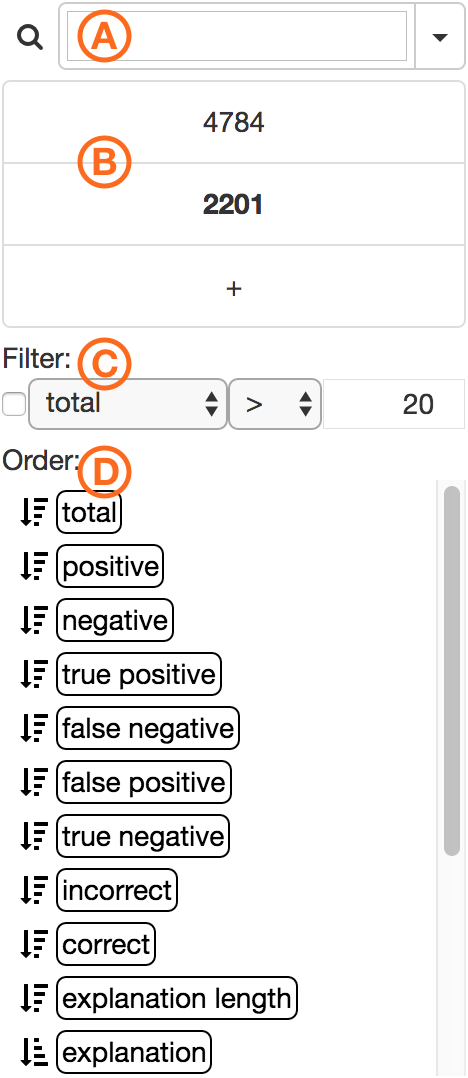
\includegraphics[width=0.45\linewidth]{fig/controls_annotated}
\caption{
The controls of the \tabB .
The first entry of the list of filtered data items (B) represents the full dataset and following entries show sizes after filter steps are applied.
The ``+" creates a new filter according to the current selection of explanations.
Explanations can be selected satisfying a condition (C) or by searching for features in the search box (A).
The sort order of explanations is defined by the list at the bottom (D).
}
\label{figs:controls}
\end{figure}



The rows shown by the \tabB can be reordered as well as filtered.
As shown in Figure~\ref{figs:expl_main}, the panel features various controls on the left hand side to accomplish those operations .
Filtering works by first selecting affected rows (either by clicking on a row or by using widgets on the left) and then clicking on the ``+" in the list of filtered data items~(Figure~\ref{figs:expl_main}B)
Each new filtering of data items creates a new entry in this list showing the current number of data items.
By selecting entries higher up in the list the user can go back to this filter.
The topmost entry always contains all data items of the entire data set.

Besides getting a filter for a given prediction score range from the \tabA there are two ways of filtering items: searching and conditioning.
The search field~(Figure~\ref{figs:expl_main}A) can be used to select rows whose explanation matches the query specified by the user.
While typing or using arrow keys suggestions for feature names are shown in a dropdown list.
Those suggestions are sorted by how often that feature appears in explanations and how closely it matches the already specified query.
The query can contain multiple features that need to appear in the explanation separated by a comma ``,".
The conditioning widget~(Figure~\ref{figs:expl_main}C) allows to filter by quantities.
% The widget consists of a check box to activate it, a dropdown list for choosing the quantity, a dropdown list to choose the comparator ($=$, $<$, or $>$), and an input field for specifying the number to compare against \aritra{this sentence provided too much interface details and can be avoided}. 



% The quantities that can be used to filter are:
% \vspace*{0.5em}
% \par \noindent \textbf{total}: the number of items explained by the given explanation
% \par \noindent \textbf{positive}: the number of items with a positive ground truth
% \par \noindent \textbf{negative}: the number of items with a negative ground truth
% \par \noindent \textbf{tp, fp, fn, tn}: the number of true / false, positive / negative items
% \par \noindent \textbf{correct / incorrect}: $tp + tn$ and $fp + fn$ respectively
% \par \noindent \textbf{accuracy}: the ratio of correctly classified items by total items
% \par \noindent \textbf{uncertainty}: $2 \; | \, \text{accuracy} - 0.5 \, |$ a measure of which subsets have a similar amount of correctly and incorrectly predicted items
% \par \noindent \textbf{precision}: the ratio of true positives by ground truth positives
% \par \noindent \textbf{explanation length}: the number of features in the explanation
% \par \noindent \textbf{odds ratio}: the odds ratio of the subset
% \par \noindent \textbf{+ / - confidence interval}: the upper / lower end of the odds ratio's confidence interval
% \vspace*{0.5em}

As shown in Figure~\ref{figs:expl_main}D, different metrics can be used to filter or reorder the list of explanations.  
A good use for the conditioning filter is to remove explanations that only explain a small subset of the data when looking for unusual or significant subsets.
The explanation rows can also be reordered using these metrics. 
The widget contains a list that shows the order in which explanations get sorted.
Each element has a symbol next to it indicating the sort direction which can be clicked on to change the sort direction.
Selecting an element brings it to the top of the list.

The metrics used for reordering are the same as those used for conditioning with the additional option of lexicographical sorting by using the feature names of the explanations.
Common metrics to use for sorting or reordering, besides total amount of items, are ``uncertainty" and ``odds ratio".
``Uncertainty" (the closeness of the odds ratio to one: $-| \log{(OR)} |$) provides a view into problematic areas of the machine learning model sometimes even unpredictable items when items with the same value configuration have different ground truth labels.
``Odds ratio", based on the computation mentioned earlier, points to especially strong predictive areas of the machine learning model.

\subsection{Item Level Inspector}
\label{sec:item_level}
The third panel~(Figure~\ref{figs:inspect_all}) allows for a more granular inspection of items explained by a given explanation set. This addresses \textbf{G4} by providing hints about the extent to which a model can be improved and if changing the data is necessary for that purpose.
% The user can access this panel by clicking on the corresponding button of an explanation in the \tabB.
The panel consists of a matrix showing the actual feature vectors of the given items.
Each row represents a unique feature vector pattern while columns represent features.
Rows can be expanded so that each row represents exactly one item.
Cells in the matrix are filled if the corresponding feature vector contains the feature represented by the column.
As rows are aggregates of multiple data items, the number of items is shown as a bar with the number indicated on the left side of the matrix.
The feature names for the columns are shown slanted on top of the matrix.
Bars behind the names show how often the feature is present.
The very first column in the matrix shows the predicted label (using the colors blue and orange) and its correctness (hatching pattern for incorrect predictions) of the given data item.
Items with the same feature vector configuration but different labels are shown in different rows.

Rows and columns can be reordered using different options, similar to \tabB.
% Similar to \tabB two widgets that define the sorting order are on the left.
One of the important reordering criteria for rows is the \textbf{feature order}, where items are ordered by seeing whether the first feature of the columns is present and then if the next feature is present, and is repeated for all the columns.
An important reordering criteria for the columns is the \textbf{relative feature importance}: the gini feature importance with respect to the current subset of data items and their predicted labels and correctness.


% \textbf{Rows} can be ordered this way by:
% \vspace*{0.5em}
% \par \noindent \textbf{feature order}: items are ordered by whether the first feature of the columns is present then the next feature and so on
% \par \noindent  \textbf{ground truth}: the ground truth of the items
% \par \noindent \textbf{predicted label}: the predicted label of the items
% \par \noindent \textbf{correctness}: whether the prediction was correct
% \par \noindent \textbf{frequency}: how often this unique feature vector pattern occurs
% \vspace*{0.5em}

% \textbf{Columns} can be ordered by:
% \vspace*{0.5em}
% \par \noindent \textbf{relative feature importance}: the gini feature importance with respect to the current subset of data items and their predicted labels and correctness
% \par \noindent \textbf{explanation}: whether the feature is part of the explanation defining the subset
% \par \noindent \textbf{frequency}: how often the feature appears in feature vectors
% \par \noindent \textbf{name}: the name of the feature
% \vspace*{0.5em}

The combination of the ``feature order" and the ``relative feature importance" criteria provide a particularly interesting view on the subset of data items.
Using this order, the most discriminating features with respect to predicted and actual labels are shown first.
Since the rows are ordered by those features, a user can follow those orderings to see how to separate different predicted and actual labels.
This guidance of the user to relevant associations in the item subset are useful for quickly understanding the raw data.
Note that it is sometimes possible to fully separate data items this way.
However, utilizing this separation would be overfitting on the validation set.
Furthermore, the opposite situation with exact same feature vectors but with different labels that cannot be separated exists as well.

Some features are not discriminative in terms of ``relative feature importance". They can be ignored to simplify the matrix view.
